\documentclass{zirkelblatt}
\geometry{tmargin=2cm,bmargin=3cm,lmargin=3cm,rmargin=3cm}
\usepackage{empheq}
\usepackage{float}
\usepackage{dashrule}
\usepackage{manfnt}
\floatstyle{ruled}
\restylefloat{figure}
\newcommand{\head}[1]{\section*{\rmfamily #1}}%begin{center}\large \textbf{#1}\end{center}}
\let\raggedsection\centering
\newcommand{\ZZ}{\mathbb{Z}}
\newcommand{\RR}{\mathbb{R}}
\newcommand{\xra}[1]{\xrightarrow{#1}}

\theoremstyle{definition}
\newtheorem{defn}{Definition}[section]
\newtheorem{axiom}[defn]{Axiom}
\newtheorem{bsp}[defn]{Beispiel}

\theoremstyle{plain}

\newtheorem{prop}[defn]{Proposition}
\newtheorem{motto}[defn]{Motto}
\newtheorem{wunder}[defn]{Wunder}
\newtheorem{ueberlegung}[defn]{Überlegung}
\newtheorem{lemma}[defn]{Lemma}
\newtheorem{kor}[defn]{Korollar}
\newtheorem{hilfsaussage}[defn]{Hilfsaussage}
\newtheorem{satz}[defn]{Satz}

\theoremstyle{remark}
\newtheorem{bem}[defn]{Bemerkung}
\newtheorem{aufg}[defn]{Aufgabe}

\definecolor{darkred}{rgb}{0.7,0,0}
\definecolor{shadecolor}{rgb}{.95,.95,.95}

\begin{document}

\maketitleSF{Klasse 11./12., Gruppe 2}{31. Mai 2014: \\ Synthetische
Differentialgeometrie}

\tableofcontents

\section{Einleitung}

Eine \emph{infinitesimale Zahl}~$\varepsilon$ ist eine Zahl, deren Quadrat Null
ist:~$\varepsilon^2 = 0$. In der gewöhnlichen mathematischen Welt gibt es nur
eine einzige infinitesimale Zahl, nämlich die Zahl~$0$. Für gewisse Anwendungen wäre es
aber schön, wenn es auch interessantere infinitesimale Zahlen gäbe. Ähnlich wie
bei den komplexen Zahlen kann man solche Zahlen \emph{künstlich} konstruieren;
anders als bei den komplexen Zahlen muss man dafür aber gleich ein ganzes neues
\emph{mathematisches Universum} errichten.

Das Teilgebiet der Mathematik, in dem man solche Universen studiert, heißt
\emph{synthetische Differentialgeometrie} und ist ein relativ junges
Forschungsgebiet. Erste Ideen gehen auf die alten Griechen und Versuche des
dänischen Mathematikers Johannes Hjelmslev zurück (*~1873, †~1950), richtig
initiiert und ausgearbeitet wurde das Gebiet aber erst in den 1970er Jahren
durch William Lawvere (Amerikaner) und Anders Kock (ebenfalls Däne). Beide sind
noch aktiv.

Im Folgenden werden wir lernen, wozu infinitesimale Zahlen nützlich sind; wie
man in dem alternativen Universum arbeiten kann; und schließlich inwieweit
Resultate, die man in der neuen mathematischen Welt erzielt, auch in der
gewöhnlichen mathematischen Welt Gültigkeit haben. Ohne diesen letzten Punkt
wäre unser Unterfangen ein reines Gedankenexperiment ohne Nutzen. Die Vorteile
von synthetischer Differentialgeometrie haben übrigens einen interessanten
Preis, den wir auch verstehen werden.

Dreh- und Angelpunkt für synthetische Differentialgeometrie ist ein Axiom,
das \emph{klassisch} -- das heißt im gewöhnlichen mathematischen Universum --
falsch ist:

\newcommand{\axiommikro}{
  \begin{shaded}
  \textbf{Axiom der Mikroaffinität.}
  Sei~$\Delta := \{ \varepsilon \in \RR \,|\, \varepsilon^2 = 0 \}$ die
  \emph{infinitesimale Monade} um~$0$. Sei~$f : \Delta \to \RR$ eine beliebige
  Funktion. Dann gibt es gewisse eindeutig bestimmte reelle Zahlen~$a$ und~$b$,
  sodass für alle Zahlen~$\varepsilon$ in~$\Delta$ folgende Gleichung gilt:
  \[ f(\varepsilon) = a + b \varepsilon. \]
  \vspace{-2.0em}%
  \end{shaded}
}
\axiommikro

Wir werden etwas Zeit benötigen, um zunächst überhaupt die Aussage dieses Axioms zu
verstehen und dann seine Konsequenzen zu überblicken. Teile des Theoriegebäudes
erarbeiten wir uns in Aufgaben. Diese solltest du also auch beim ersten Lesen
nicht überfliegen.

\paragraph{\textcolor{darkred}{Warnung.}} Ab einer bestimmten Stelle werden wir
leicht andere logische Gesetze verwenden als in der Schule. Insbesondere werden
deine Lehrer vielleicht nicht erfreut sein, wenn du sie in Hausaufgaben oder
Prüfungen verwendest.

\section{Motivation für infinitesimale Zahlen}

\paragraph{Schnitte.} In Abbildung~\ref{fig:schnittverhalten} sind zwei Situationen skizziert, bei
denen sich jeweils zwei Kurven schneiden. (Gerade Linien zählen
auch als \emph{Kurven}.) Es ist offensichtlich, dass sich im ersten
Bild die beiden Geraden in genau einem Punkt schneiden. Die Schnittsituation
beim zweiten Bild ist dagegen weniger klar. In klassischer Mathematik konstatiert man,
der Schnitt bestehe ebenfalls aus nur genau einem Punkt, nämlich dem Ursprung.
In der Tat könnte man keinen weiteren Punkt benennen, der ebenfalls auf beiden
Kurven liegen würde. Anschaulich scheint es aber ja doch einen Unterschied zu
geben -- man benötigt infinitesimale Zahlen, um ihn auf direkte Art und Weise
mathematisch einzufangen.\footnote{Indirekt geht es auch in klassischer
Mathematik: Die Parabel hat bei der Stelle~$x = 0$ eine \emph{doppelte
Nullstelle}. Das bedeutet, dass nicht nur der Funktionswert dort Null ist,
sondern auch noch seine erste Ableitung.}

\begin{aufgabeShaded}{Schnittberechnung I}
\label{aufg:schnittberechnung1}
Die Gleichungen der beiden Kurven im ersten Bild sind
\begin{empheq}[left=\empheqlbrace\ ]{align}
  y &= 2x, \\
  y &= 0.
\end{empheq}
Die erste Gleichung gehört zur schrägen Gerade, die zweite zur~$x$-Achse (auf
der alle Punkte als~$y$-Koordinate Null haben). Die Gleichungen der Kurven im
zweiten Bild sind
\begin{empheq}[left=\empheqlbrace\ ]{align}
  y &= x^2, \\
  y &= 0.
\end{empheq}
\begin{enumerate}
\item Löse das erste Gleichungssystem, um zu beweisen: Der einzige
Schnittpunkt~$(x|y)$ hat die Koordinaten~$x = 0$ und~$y = 0$. Wieso entspricht
das Schneiden der beiden Kurven rechnerisch der Lösungsmenge des kombinierten
Gleichungssystems?
\item Löse das zweite Gleichungssystem, um zu beweisen, dass ein Punkt~$(x|y)$
genau dann im Schnittbereich des zweiten Bilds liegt, wenn seine~$x$-Koordinate
Null und seine~$y$-Koordinate eine infinitesimale Zahl ist (also~$y^2 = 0$
erfüllt).

Hierbei ist es wichtig, mit Absicht langsam zu rechnen, um nicht durch zu
schnelles Vereinfachen die Pointe vorwegzunehmen. In klassischer Mathematik
gilt die Regel "`wenn~$y^2 = 0$, dann auch~$y = 0$"'; erst mit dieser Regel
vereinfacht sich das Ergebnis, dann zu demselben wie in Teilaufgabe~a).
\end{enumerate}
\end{aufgabeShaded}

\paragraph{Physik.} Infinitesimale Zahlen sind ferner in der Physik nützlich. Dort hat man es
manchmal mit "`sehr kleinen"' (aber nicht verschwindenden) Größen wie etwa
Differenzen~$\Delta x$ zu tun. Da das Quadrat einer kleinen Zahl nochmals
kleiner und "`wirklich winzig"' ist, erlaubt man sich, in Rechnungen Quadrate
von~$\Delta x$ einfach wegzulassen. Das ist mathematisch natürlich nicht
zulässig -- trotzdem haben die Physikerinnen und Physiker mit diesem Vorgehen
offensichtlich großen Erfolg!

Mathematiker sollten die physikalischen Methoden nicht blind verurteilen,
sondern sie ernst nehmen und Möglichkeiten finden, sie mathematisch sauber und
rigoros zu verstehen. Infinitesimale Zahlen bieten eine solche Möglichkeit.sie
ernst nehmen und Möglichkeiten finden, sie mathematisch sauber und rigoros zu
verstehen. Infinitesimale Zahlen bieten eine solche Möglichkeit.

\begin{aufgabeShaded}{Quadrate großer und kleiner Zahlen}
\begin{enumerate}
\item Sei~$x$ eine reelle Zahl, die größer als~$1$ ist. Zeige: Das
Quadrat~$x^2$ ist größer als~$x$.
\item Sei~$x$ eine reelle Zahl zwischen~$0$ und~$1$. Zeige: Das Quadrat~$x^2$
ist kleiner als~$x$.

Wenn die Dezimalentwicklung von~$x$ mit~$n$ Nullen nach dem Komma beginnt, mit
etwa wie vielen Nullen beginnt dann die Dezimalentwicklung von~$x^2$?
\end{enumerate}
\end{aufgabeShaded}

\paragraph{Differentialrechnung.}
Infinitesimale Zahlen sind ferner fürs Differenzieren nützlich: Sie ermöglichen
es nämlich, auf gewisse Grenzwertprozesse zu verzichten und gleichzeitig näher
an der Anschauung zu bleiben. Zur Erinnerung wollen wir die übliche Definition
der Ableitung rekapitulieren:

\begin{defn}Sei~$f : \RR \to \RR$ eine Funktion und~$x_0 \in \RR$ eine Stelle.
Falls der Grenzwert
\[ \lim_{\varepsilon \to 0} \frac{f(x_0 + \varepsilon) - f(x_0)}{\varepsilon} \]
existiert, so heißt~$f$ an der Stelle~$x_0$ \emph{differenzierbar} und die
Ableitung~$f'(x_0)$ ist per Definition dieser Grenzwert.
\end{defn}

\begin{aufgabeShaded}{Intuition zum Differentialquotienten}
Erinnere dich, inwieweit der Bruch
\[ \frac{f(x_0 + \varepsilon) - f(x_0)}{\varepsilon} \]
für festes~$\varepsilon$ eine \emph{Sekantensteigung} angibt, und erkläre anhand einer Skizze, wieso der
Grenzwert für~$\varepsilon \to 0$ anschaulich die Steigung der Tangente an den
Graphen von~$f$ durch den Punkt~$(x_0|f(x_0))$ angibt.
\end{aufgabeShaded}

Um die Definition besser zu verstehen, möchten wir ohne Verwendung der bekannten
Ableitungsregeln die Ableitung der Quadratfunktion bestimmen.

\begin{prop}Die Quadratfunktion~$f : \RR \to \RR,\,x \mapsto x^2$ ist überall
differenzierbar mit Ableitung~$f'(x) = 2x$.\end{prop}
\begin{proof}In der Schule würde man in einer langen Gleichungskette die
Definition so lange vereinfachen, bis der Grenzwert unmittelbar ablesbar ist.
Dabei müsste man in jedem Schritt das~$\lim$-Symbol mitführen, würde das aber
vielleicht auch oftmals vergessen. Übersichtlicher ist folgende Schreibweise:
\[ \frac{f(x + \varepsilon) - f(x)}{\varepsilon} =
  \frac{(x + \varepsilon)^2 - x^2}{\varepsilon} =
  \frac{x^2 + 2x\varepsilon + \varepsilon^2 - x^2}{\varepsilon} =
  2x + \varepsilon \xra{\varepsilon \to 0} 2x. \qedhere \]
\end{proof}

An diesem Beweis ist an sich nichts auszusetzen. Die Rechnung selbst ist genügend
einfach, durch die Grenzwertüberlegung aber trotzdem logisch nicht ganz
elementar. Die Physiker haben eine einfachere Möglichkeit, die Aussage zu
"`beweisen"' -- eine, die ohne Grenzwerte auskommt:

\begin{proof}[Physiker-Beweis]Sei~$\varepsilon$ "`sehr klein"'. Dann gilt:
\[ \frac{f(x + \varepsilon) - f(x)}{\varepsilon} =
  \frac{(x + \varepsilon)^2 - x^2}{\varepsilon} =
  \frac{x^2 + 2x\varepsilon + \varepsilon^2 - x^2}{\varepsilon} =
  2x + \varepsilon = 2x. \qedhere \]
\end{proof}

Bemerkenswert ist die schizophrene Natur dieses Arguments:
Zum einen lässt man im letzten Schritt den Term~$\varepsilon$ einfach weg --
mit der Begründung,~$\varepsilon$ sei schließlich "`sehr klein"'. Andererseits
aber teilt man durch~$\varepsilon$ -- das ginge nur, wenn man wüsste,
dass~$\varepsilon$ positiv oder negativ, aber jedenfalls nicht Null ist.

Außerdem sollte man auch zu Beginn der Rechnung die Vereinfachung~$f(x +
\varepsilon) - f(x) = f(x) - f(x) = 0$ treffen dürfen, wenn man doch am Ende
ebenfalls einfach~$\varepsilon$ weglassen durfte. Schließlich sollten sich die
Rechengesetze nicht inmitten einer Rechnung ändern. Dann wäre das Ergebnis
insgesamt~$f'(x) = 0$ -- das ist jedoch eine unsinnige Behauptung.

Aus diesen Gründen wird das Physiker-Argument in klassischer Mathematik
nicht akzeptiert. Mit den infinitesimalen Zahlen aus synthetischer
Differentialgeometrie werden wir aber in der Lage sein, die wesentlichen Ideen des
Physiker-Arguments in einen mathematisch einwandfreien Beweis zu gießen. So
können wir die Vorteile beider Welten -- einfache Rechnungen einerseits und
mathematische Rigorosität andererseits -- vereinen.

\begin{aufgabeShaded}{Ableitung der Kubikfunktion I}
Sei~$f : \RR \to \RR,\,x \mapsto x^3$ die Kubikfunktion. Verifiziere direkt
anhand der mathematischen Definition, dass~$f$ überall differenzierbar mit
Ableitung~$f'(x) = 3x^2$ ist.

\emph{Hinweis:} Den Ausdruck~$(x + \varepsilon)^3$ kann man entweder durch
mehrmaliges Ausmultiplizieren oder direkt durch Verwendung der binomischen
Formel für Kuben statt Quadrate vereinfachen. (Die Koeffizienten der
allgemeinen binomischen Formel stehen im Pascalschen Dreieck.)
\end{aufgabeShaded}

\begin{aufgabeShaded}{Beispiele für nicht differenzierbare Funktionen}
\label{aufg:nichtdb}
\begin{enumerate}
\item Die Betragsfunktion (siehe Abbildung~\ref{fig:nicht-diffbar}a) ist an der
Stelle~$x_0 = 0$ nicht differenzierbar. Anschaulich erkennt man das daran, dass
der Graph am Punkt~$(0|0)$ keine eindeutige Tangente besitzt.\footnotemark{}
Bestätige diese Beobachtung anhand der Definition über den
Differentialquotienten: Die Sekantensteigungen konvergieren für~$\varepsilon
\to 0$ nicht gegen einen bestimmten Wert, sondern \ldots

Wenn du möchtest, kannst du das auch noch rechnerisch nachvollziehen: Berechne
den \emph{links-} und den \emph{rechtsseitigen} Grenzwert des
Differenzenquotienten. Nutze dazu folgende Definition der Betragsfunktion:
\[ |x| := \begin{cases}\phantom{-}x, & \text{falls $x \geq 0$,} \\ -x, & \text{falls $x <
0$.}\end{cases} \]
\item Es gibt auch Funktionen, deren Graphen keine offensichtlichen
Knickpunkte haben und die trotzdem nicht überall differenzierbar sind. Erkläre
anschaulich und zeige rechnerisch, dass folgende Funktion an der Stelle~$x_0 =
0$ nicht differenzierbar ist (siehe Abbildung~\ref{fig:nicht-diffbar}b):
\[ f(x) = \begin{cases}x \sin\frac{1}{x}, & \text{falls $x \neq 0$,} \\
0, & \text{falls $x = 0$.}\end{cases} \]
(Diese Funktion ist übrigens durchaus \emph{stetig}.)
\end{enumerate}
\end{aufgabeShaded}
\footnotetext{Man kann an dieser Stelle durchaus Geraden anlegen, es gibt aber
keine besonders überzeugende Wahl einer \emph{berührenden} Gerade.
Fortgeschrittene Differentialrechnung wird mit dieser Uneindeutigkeit fertig,
durch den Begriff der \emph{Subgradienten} von konvexen Funktionen.}


\section{Exkurs zu Mengen und Funktionen}

Eine \emph{Menge} reeller Zahlen kann man sich wie eine Einkaufstasche
vorstellen, die statt leckerer Äpfel gewisse reelle Zahlen enthält. Die Zahlen,
die in einer Menge vorkommen, heißen \emph{Elemente} dieser Menge. Mengen
dürfen auch unendlich viele oder gar keine Elemente enthalten. Es gibt drei
Möglichkeiten, Mengen anzugeben:
\begin{align*}
  M_1 &= \{ 4, 9, 16, 25, 36, 49, 64, 81 \}, \\
  M_2 &= \{ 4, 9, 16, \ldots, 81 \}, \\
  M_3 &= \{ x \in \RR \ |\ \text{$x \geq 4$ und $x \leq 81$ und $x$ ist das Quadrat
  einer natürlichen Zahl} \}.
\end{align*}
Im ersten Fall zählt man die Elemente der Menge einfach explizit auf. Im
zweiten Fall erwartet man von seinem Gegenüber, die Regelmäßigkeit zu erkennen
und die in der Notation nicht aufgeführten Elemente gedanklich zu ergänzen. Der
dritte Fall liest sich wie folgt: Die Menge~$M_3$ ist die Menge all derjenigen
reellen Zahlen ("`$x \in \RR$"'), welche~$\geq 4$, $\leq 81$ und zugleich das
Quadrat einer natürlichen Zahl sind; man sammelt also alle reellen Zahlen mit
einer gewissen Eigenschaft auf.

\begin{aufgabeShaded}{Beispiele für Mengen}
Sei~$M = \{ x \in \RR \ |\ x^2 \geq 4 \}$. Skizziere die Menge~$M$ auf dem
Zahlenstrahl.
\end{aufgabeShaded}

Eine \emph{Funktion}~$f : D \to \RR$ ordnet jedem Element ihrer
\emph{Definitionsmenge}~$D$ eine bestimmte reelle Zahl zu: Liegt~$x$ in~$D$, so
ist~$f(x)$ eine bestimmte reelle Zahl. Für Zahlen~$x$ außerhalb der
Definitionsmenge ist~"`$f(x)$"' ein sinnloser Ausdruck.

Zuordnungen wie~$f : x \mapsto \pm x$, für die~$f(x)$ gewissermaßen
mehrere Werte annimmt, führen nicht zu Funktionen, sondern zu \emph{Relationen}.
Solche werden wir im Folgenden nie betrachten.

\begin{aufgabeShaded}{Funktionen mit eingeschränkten Definitionsmengen}
\begin{enumerate}
\item Finde die größtmögliche Definitionsmenge~$D$, sodass folgende Zuordnung
Sinn ergibt:
\[ f : D \to \RR,\,x \mapsto \frac{1}{x}. \]
\item Der Term~"`$x^2$"' ergibt für alle reellen Zahlen~$x$ Sinn, die
größtmögliche Definitionsmenge der Zuordnung~$x \mapsto x^2$ ist also die
vollständige Menge~$\RR$ aller reellen Zahlen. Man kann aber die
Definitionsmenge auch künstlich einschränken:
\[ f : [2;4] \to \RR,\,x \mapsto x^2. \]
Dabei bezeichnet~"`$[2;4]$"' das abgeschlossene Intervall von~$2$ bis~$4$, also
die Menge~$\{ x \in \RR \,|\, 2 \leq x \leq 4 \}$. Skizziere den Verlauf dieser
Funktion. (Das wird \emph{nicht} die übliche Normalparabel.)
\end{enumerate}
\end{aufgabeShaded}


\section{Das Axiom der Mikroaffinität}

Im Axiom der Mikroaffinität kommt die \emph{infinitesimale Monade um die
Zahl~$0$} vor. Damit ist folgende Menge reeller Zahlen gemeint:
\[ \Delta := \{ x \in \RR \,|\, x^2 = 0 \}. \]
Die Elemente von~$\Delta$ sind also all diejenigen Zahlen, deren Quadrat Null
ist. In klassischer Mathematik gilt die Regel "`wenn das Quadrat einer Zahl
Null ist, dann ist auch die Zahl selbst Null"'. Daher besteht~$\Delta$ in klassischer
Mathematik nur aus der Zahl~$0$: $\Delta = \{ 0 \}$.

Da wir uns in Kürze von klassischer Mathematik (vorläufig) verabschieden
möchten, geben wir nun genau an, welche der Axiome klassischer Mathematik wir
noch verwenden möchten:
\begin{itemize}
\item Die üblichen logischen Gesetze -- mit einer wichtigen Ausnahme, die wir
in Abschnitt~\ref{sect:lem} diskutieren werden.

Ein logisches Gesetz ist etwa: Wenn sowohl eine Aussage~$A$
als auch eine Aussage~$B$ stimmen, so stimmt insbesondere~$A$. Ein anderes
lautet: Wenn eine Aussage~$A$ stimmt und~$B$ eine weitere (vielleicht falsche)
Aussage ist, so stimmt es auch, dass~$A$ oder~$B$ korrekt ist.\footnote{In der
Mathematik ist "`oder"' stets einschließend gemeint, wenn man nicht mit
"`entweder oder"' explizit die ausschließende Variante verwendet. Wenn ich
also heute Abend ins Kino gehen \emph{und} später schlafen werde, so stimmt es
insbesondere auch, dass ich heute Abend ins Kino gehen \emph{oder} schlafen
werde.}
\item Die üblichen Rechenregeln zur Termvereinfachung.
\begin{align*}
  0 + x &= x &
  1 \cdot x &= x \\
  x + y &= y + x &
  x \cdot y &= y \cdot x \\
  x + (y + z) &= (x + y) + z &
  x \cdot (y \cdot z) &= (x \cdot y) \cdot z
\end{align*}
\begin{align*}
  x \cdot (y + z) &= x \cdot y + x \cdot z \\
  (x + y) \cdot z &= x \cdot z + y \cdot z
\end{align*}
\item Das Axiom zu Gegenzahlen: Jede reelle Zahl besitzt eine zugehörige
Gegenzahl -- zu~$x$ gibt es eine Zahl~$-x$ mit der Eigenschaft~$x + (-x) = 0$.
\item Das Axiom zu Inversen: Ist eine reelle Zahl \emph{nicht Null}, so besitzt
sie ein Inverses bezüglich der Multiplikation. In Formeln: Wenn~$x \neq 0$, so
gibt es eine Zahl~$y$ mit~$xy = 1$. Das Inverse~$y$ wird üblicherweise
als~"`$\frac{1}{x}$"' oder~"`$x^{-1}$"' geschrieben.
\item Ein \emph{Nichttrivialitätsaxiom}: $0 \neq 1$.
\item Einige weitere Axiome, die wir aber erst dann einführen, wenn wir sie
benötigen. Es sei nur noch verraten, dass wir die \emph{Trichotomie} der Ordnung
\emph{nicht} verwenden: Diese würde besagen, dass jede Zahl entweder kleiner,
gleich oder größer als Null ist.
\end{itemize}

Diese Axiome rechtfertigen jedenfalls \emph{nicht} die Regel, der zufolge das
Quadrat einer Zahl nur dann Null sein könne, wenn sie es selbst schon wäre.
Auch wenn wir keine weiteren Elemente in~$\Delta$ angeben können, können wir
mit unserem reduzierten Satz an Axiomen daher trotzdem nicht schließen,
dass~$\Delta$ \emph{nur} die Null enthalte.

Wir stellen uns die Menge~$\Delta$ als eine \emph{infinitesimale Umgebung} der
Zahl~$0$ vor. Keine konkrete kleine positive Zahl liegt in~$\Delta$ -- etwa
liegt ein Millionstel nicht in~$\Delta$, denn das Quadrat eines Millionstels
ist nicht Null, sondern ein Billionstel. Wir stellen uns~$\Delta$ eher als die
Menge der ($x$-Koordinaten der) Schnittpunkte in Abbildung~\ref{fig:schnittverhalten}b vor.

Mathematisch erweckt das Axiom der Mikroaffinität die Menge~$\Delta$ zum Leben
und bestätigt dann unsere Intuition über~$\Delta$. Sobald wir dieses Axiom
annehmen, verlassen wir klassische Mathematik.

\textcolor{darkred}{\hspace{-5cm}\hdashrule{2\textwidth}{1pt}{3mm}}

\axiommikro
\begin{figure}[b]
  \centering
  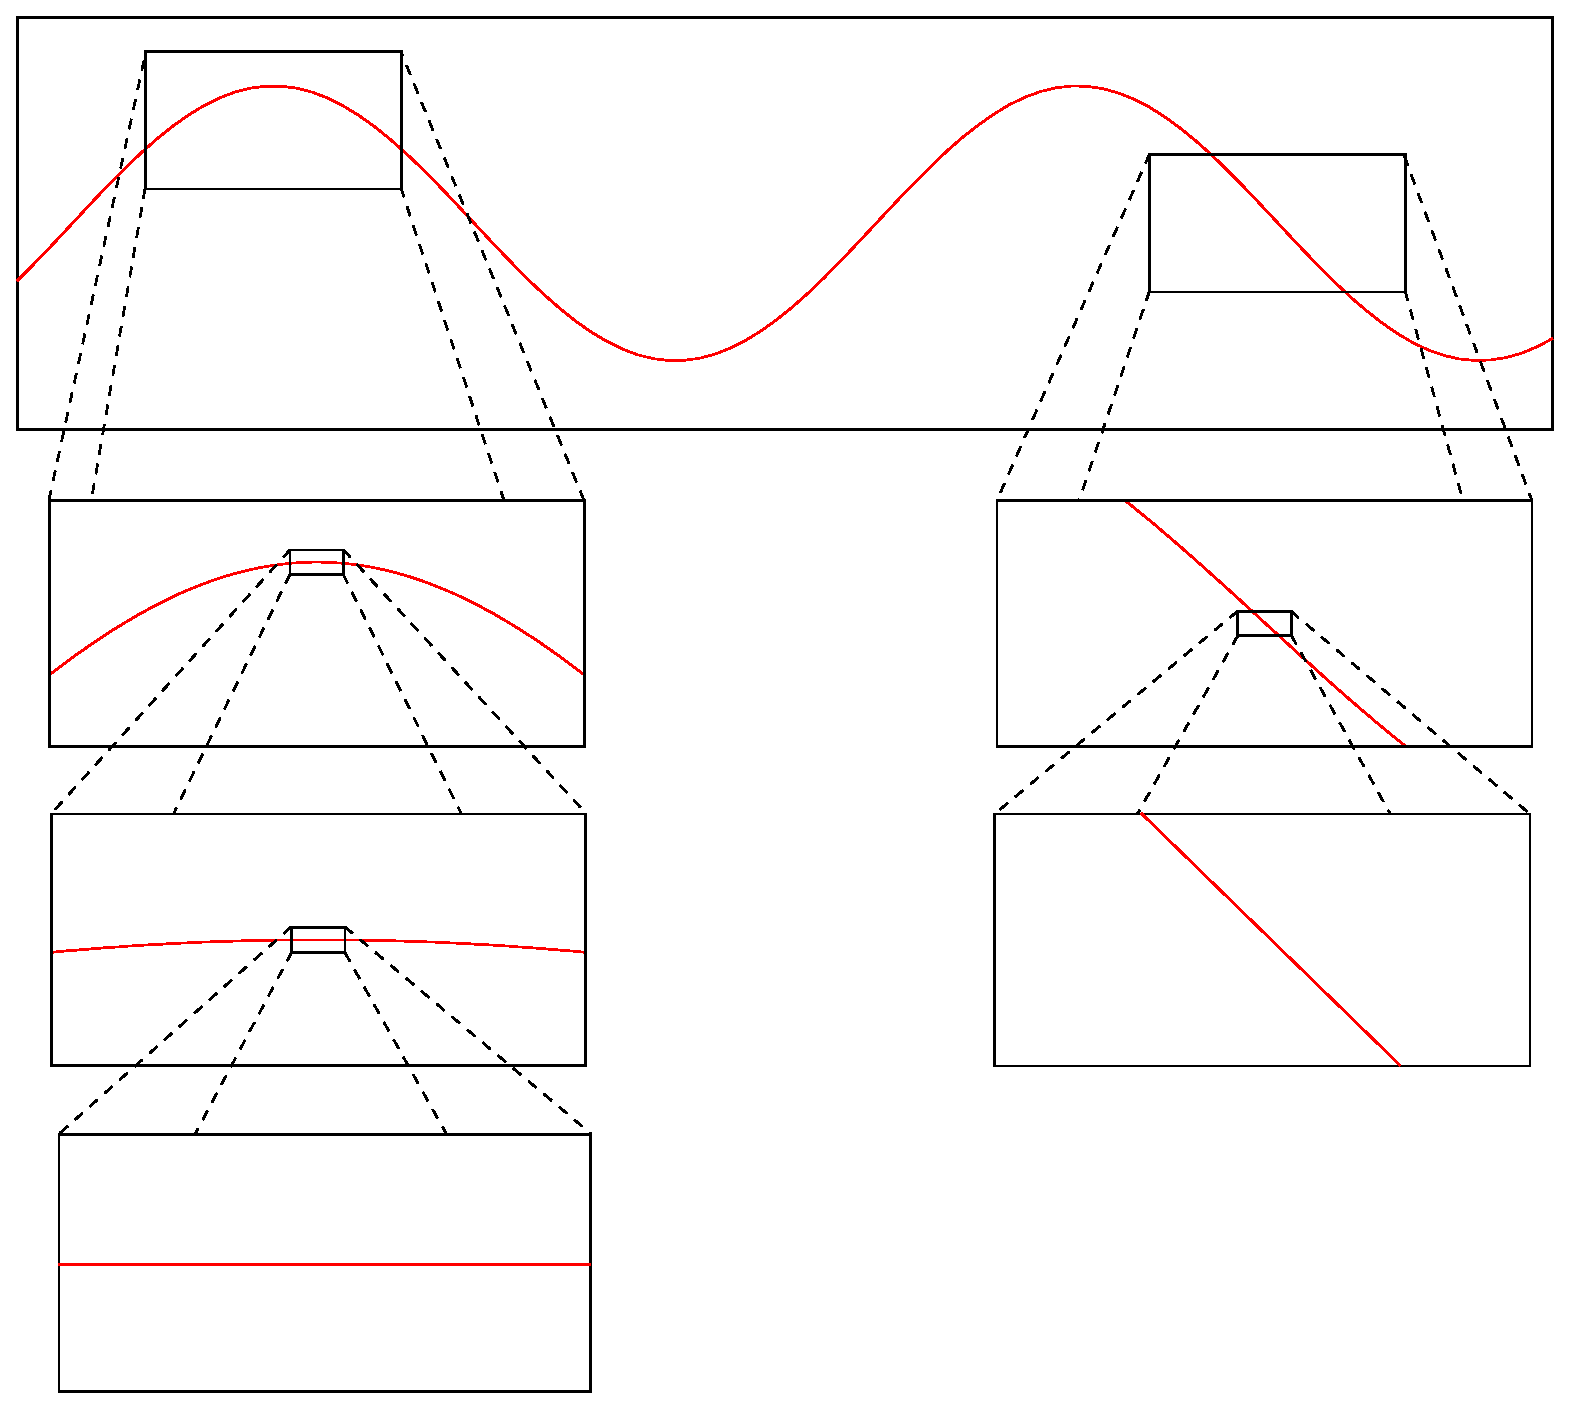
\includegraphics[width=\textwidth]{mikroaffinitaet}
  \caption{Auf infinitesimalen Umgebungen sind Funktionen affin.}
\end{figure}
% http://upload.wikimedia.org/wikipedia/commons/f/fa/Approximation_of_cos_with_linear_functions_without_numbers.svg

Das Axiom spricht nicht über Funktionen~$\RR \to \RR$, sondern nur
über solche, deren Definitionsmengen die infinitesimale Monade~$\Delta$ sind.
Die Funktionswerte einer solchen Funktion können also nur in sehr begrenzten
Ausmaßen variieren. Das Axiom besagt nun: Eine solche Funktion sieht stets wie
eine affine Funktion aus, mit Achsenabschnitt~$a$ und Steigung~$b$.\footnote{In
der Schule nennt man solche Funktionen \emph{linear}. In Universitätsmathematik
ist dieser Begriff nur solchen affinen Funktionen vorbehalten, deren
Achsenabschnitt Null ist.}

Zu betonen ist auch, dass laut Axiom Achsenabschnitt~$a$ und Steigung~$b$ \emph{eindeutig
bestimmt} sind. Das bedeutet: Sollte für eine Funktion~$f : \Delta \to \RR$
nicht nur~$f(\varepsilon) = a + b\varepsilon$, sondern auch~$f(\varepsilon) =
\tilde a + \tilde b \varepsilon$ für alle~$\varepsilon$ in~$\Delta$ gelten, so
folgt~$a = \tilde a$ und~$b = \tilde b$.

Eine erste Konsequenz des Mikroaffinitätsaxioms ist, dass die Menge~$\Delta$
anders als in klassischer Mathematik nicht nur die Null enthält.
\begin{prop}\label{prop:neg-delta0}Es stimmt nicht, dass~$\Delta = \{ 0 \}$.\end{prop}
\begin{proof}Angenommen, es wäre doch der Fall, dass~$\Delta = \{ 0 \}$. Dann
erhalten wir mit der Eindeutigkeitsaussage im Axiom der Mikroaffinität einen
Widerspruch: Betrachte die Funktion $f : \Delta \to \RR,\,\varepsilon \mapsto 0$.
Dann gelten für alle~$\varepsilon$ in~$\Delta$ -- das ist etwas verklausuliert
gesprochen, denn nach Annahme enthält~$\Delta$ ja nur die Null -- \emph{beide}
der folgenden Gleichungen:
\begin{align*}
  f(\varepsilon) &= 0 + 0 \cdot \varepsilon \\
  f(\varepsilon) &= 0 + 1 \cdot \varepsilon
\end{align*}
Wegen der Eindeutigkeitssaussage müsste daher~$0 = 1$ sein. Das ist aber ein
Widerspruch zum Axiom~$0 \neq 1$.
\end{proof}

Wir sind hier also in einer etwas sonderbaren Situation: In klassischer
Mathematik gilt~$\Delta = \{ 0 \}$, das Axiom der Mikroaffinität impliziert
aber~$\Delta \neq \{ 0 \}$. Andererseits können wir trotzdem keine Zahl
in~$\Delta$ (außer der Null) explizit angeben. Beide Paradoxien müssen wir
auflösen, um wieder produktiv arbeiten zu können. Zunächst aber wollen wir ein
paar Rechnungen anstellen, um den Umgang mit dem Axiom der Mikroaffinität zu
üben. \dbend

\begin{aufgabeShaded}{Eine erste korrekte Rechnung mit infinitesimalen Zahlen}
\label{aufg:erste-rechnung}
Sei~$\varepsilon$ eine Zahl in~$\Delta$. Vereinfache dann den Ausdruck
\[ (x + \varepsilon)^2 - x^2 \]
so weit wie möglich. Das geht ähnlich wie bei unserer Berechnung der Ableitung
der Quadratfunktion. Am Ende wird ein~$\varepsilon$ stehen bleiben.

Das Axiom der Mikroaffinität wirst du dazu noch nicht benötigen -- aber ohne es
wäre die Rechnung langweilig, denn dann wäre ja~$\varepsilon = 0$ die einzige
infinitesimale Zahl.
\end{aufgabeShaded}

\begin{aufgabeShaded}{Magneteigenschaft infinitesimaler Zahlen}
Die infinitesimalen Zahlen haben folgende \emph{Magneteigenschaft}: Das Produkt
einer beliebigen Zahl mit einer infinitesimalen Zahl ist wieder eine
infinitesimale Zahl.

Beweise das! Sei dazu~$x$ eine beliebige reelle Zahl und~$\varepsilon$ eine
infinitesimale Zahl, also eine solche, deren Quadrat Null ist. Zeige dann,
dass~$x \cdot \varepsilon$ ebenfalls infinitesimal ist.
\end{aufgabeShaded}

\begin{aufgabeShaded}{Invertierbarkeit infinitesimaler Zahlen}
Infinitesimale Zahlen sind nicht so weit von der Null verschieden, als dass sie
invertierbar sein könnten. Das wollen wir in dieser Aufgabe beweisen. Ergänze
folgenden Beweisanfang:

\emph{Sei~$\varepsilon$ in~$\Delta$. Angenommen,~$\varepsilon$ wäre
doch invertierbar. Nach Definition der Invertierbarkeit würde es dann eine weitere
Zahl~$y$ mit der Eigenschaft~$\varepsilon \cdot y = 1$ geben. Dann \ldots}
\end{aufgabeShaded}

\begin{aufgabeShaded}{Das Prinzip der Mikrokürzbarkeit}
\label{aufg:mikrokuerzbarkeit}
\begin{enumerate}
\item Sei~$x$ eine invertierbare reelle Zahl (das heißt, dass es eine Zahl~$y$
mit~$xy = 1$ gibt). Seien ferner~$a$ und~$b$ reelle Zahlen. Zeige:
\[ \text{Wenn $xa = xb$, dann $a = b$.} \]
Invertierbare Zahlen kann man also in Gleichungen kürzen. Das ist für dich
natürlich nichts Neues, vielleicht ist das aber das erste Mal, dass du einen
Beweis dieser elementaren Tatsache geführt hast.

\item In manchen Zahlenbereichen gibt es auch Zahlen, die nicht invertierbar,
aber trotzdem aus Gleichungen kürzbar sind. Fällt dir etwa ein Beispiel im
Bereich der ganzen Zahlen~$\ZZ$ ein?

\item Ob einzelne infinitesimale Zahlen kürzbar sind oder nicht, können wir mit
den gegebenen Axiomen nicht entscheiden. (Sicherlich sind nicht alle
infinitesimale Zahlen kürzbar, denn die Null ist ja auch eine infinitesimale
Zahl.) Es gilt jedoch folgendes Prinzip der \emph{Mikrokürzbarkeit}:
\[ \text{Wenn~$\varepsilon a = \varepsilon b$ für \emph{alle} $\varepsilon$
in~$\Delta$, dann $a = b$.} \]
Beweise dieses Prinzip! Dazu wirst du das Axiom der Mikroaffinität verwenden
und eine geeignete Hilfsfunktion~$f : \Delta \to \RR$ definieren müssen.
\end{enumerate}
\end{aufgabeShaded}

\begin{aufgabeShaded}{Schnittberechnung II}
Auf der~$x$-Achse ruhe ein Kreis mit Radius~$1$ und Mittelpunkt~$(0|1)$.
Überprüfe rechnerisch, dass die Schnittpunkte von Kreis und~$x$-Achse genau die
folgenden sind:~$(\varepsilon|0)$ mit~$\varepsilon$ in~$\Delta$.

Dieses Beispiel stammt übrigens vom griechischen Philosophen Protagoras
(*~vermutlich um~490\,v.\,Chr., †~vermutlich um~411\,v.\,Chr.). Er
war der Auffassung, der Schnitt bestehe nicht nur aus einem einzelnen Punkt,
sondern einem \emph{infinitesimalen Geradenstück}. Deine Rechnung wird diese
Auffassung bestätigen.

\emph{Tipp:} Schlage die \emph{Kreisgleichung} auf Wikipedia nach oder leite
sie mit dem Satz des Pythagoras her. Die Rechnung selbst ist dann ähnlich wie
bei Aufgabe~\ref{aufg:schnittberechnung1}.
\end{aufgabeShaded}


\section{Differentialrechnung mit infinitesimalen Zahlen}

Die Ableitung von Funktionen können wir mit dem Axiom der Mikroaffinität
deutlich leichter einführen.

\begin{defn}\label{defn:sdg-ableitung}
Sei~$f : \RR \to \RR$ eine Funktion. Sei~$x_0 \in \RR$ eine Stelle.
Dann heißt die eindeutig bestimmte Zahl~$b$, für die für alle~$\varepsilon$
in~$\Delta$ die Gleichung
\[ f(x_0 + \varepsilon) = f(x_0) + b\varepsilon \]
gilt, die \emph{Ableitung von~$f$ an der Stelle~$x_0$}. Wir schreiben dann
auch~"`$f'(x_0)$"' für diese Zahl~$b$.\end{defn}

Abbildung~\ref{fig:ableitung-sdg} illustriert die Intuition hinter dieser
Definition: In einer infinitesimalen Umgebung von~$x_0$ sieht der Graph von~$f$
wie eine Gerade aus, nämlich genauer wie die Tangentialgerade durch den
Punkt~$(x_0|f(x_0))$. Also sieht auch der Term~$f(x_0 + \varepsilon)$ wie der
Term einer affinen Funktion aus: An der Stelle~$\varepsilon = 0$ hat er den
Wert~$f(x_0)$, für andere infinitesimale~$\varepsilon$ weicht er von~$f(x_0)$
um~$b \varepsilon$ ab.

Wir werden die definierende Gleichung oft in folgender umgestellten Form
verwenden:
\[ f'(x_0) \cdot \varepsilon = f(x_0 + \varepsilon) - f(x_0). \]

Die Definition ist nur dann sinnvoll, wenn garantiert ist, dass es eine
solche Zahl~$b$ wirklich gibt und dass sie \emph{eindeutig} ist, dass es also
auch \emph{nur} eine solche Zahl gibt. Daher müssen wir folgende Aufgabe
bearbeiten.

\begin{aufgabeShaded}{Sinn der neuen Ableitungsdefinition}
Verwende das Axiom der Mikroaffinität, um zu zeigen, dass eine Zahl~$b$ wie in
Definition~\ref{defn:sdg-ableitung} gibt und dass sie eindeutig ist. Dazu wirst
du eine gewisse Hilfsfunktion~$g : \Delta \to \RR$ definieren müssen.
\end{aufgabeShaded}

Die Definition offenbart übrigens ein weiteres Paradox: In klassischer
Mathematik gibt es ja auch Funktionen, die nicht differenzierbar sind, etwa
weil sie wie die Betragsfunktion Knickstellen besitzen (siehe
Aufgabe~\ref{aufg:nichtdb}). Hier aber ist \emph{jede}
Funktion differenzierbar! Auch dieses Paradox werden wir zu gegebener Zeit
auflösen. \dbend

Wir haben jetzt die Technologie so weit entwickelt, um mit Hilfe
infinitesimaler Zahlen Funktionen auf einfache Art und Weise ableiten zu
können. Das wollen wir zunächst an der Quadratfunktion illustrieren.

\begin{prop}\label{prop:ableitung-quadratfunktion-sdg}
Die Ableitung der Quadratfunktion~$f : \RR \to \RR,\,x \mapsto x^2$
ist~$f'(x) = 2x$.\end{prop}
\begin{proof}Für alle~$\varepsilon$ in~$\Delta$ gilt folgende Rechnung:
\[ f'(x) \cdot \varepsilon =
  f(x + \varepsilon) - f(x) =
  \text{\ldots{} siehe Aufgabe~\ref{aufg:erste-rechnung} \ldots} =
  2x\varepsilon. \]
Da diese Rechnung für alle~$\varepsilon$ in~$\Delta$ gilt, können wir nach dem
Prinzip der Mikrokürzbarkeit (Aufgabe~\ref{aufg:mikrokuerzbarkeit}) die
Behauptung folgern: $f'(x) = 2x$.
\end{proof}

\begin{aufgabeShaded}{Ableitung der Kubikfunktion II}
Leite nach demselben Muster wie in
Proposition~\ref{prop:ableitung-quadratfunktion-sdg} die Kubikfunktion~$x
\mapsto x^3$ ab.
\end{aufgabeShaded}

\begin{aufgabeShaded}{Ableitung der Kehrwertfunktion}
Sei~$f : \RR \setminus \{0\} \to \RR,\,x \mapsto \frac{1}{x}$ die
Kehrwertfunktion. Bestimme nach demselben Muster wie in
Proposition~\ref{prop:ableitung-quadratfunktion-sdg} ihre Ableitung.
Das Ergebnis sollte natürlich~$f'(x) = -\frac{1}{x^2}$ sein.

\emph{Hinweis:} Klammere~$\frac{1}{x}$ aus. An einer Stelle wirst du die Vereinfachungsregel
\[ \frac{1}{1 + \frac{\varepsilon}{x}} = 1 - \frac{\varepsilon}{x} \]
benötigen.\footnotemark{}
Beweise diese Regel, indem du die Probe durchführst:
\[ (1 + \tfrac{\varepsilon}{x}) \cdot (1 - \tfrac{\varepsilon}{x}) = \cdots = 1. \]
\end{aufgabeShaded}

\begin{aufgabeShaded}{Ableitungsregeln}
In klassischer Mathematik sind die Summen-, Produkt- und Kettenregel sehr
nützlich. Diese gibt es auch in synthetischer Differentialgeometrie. In dieser
Aufgabe möchten wir sie mit Hilfe infinitesimaler Zahlen beweisen.

Seien also~$f$ und~$g$ Funktionen~$\RR \to \RR$. Zeige:
\begin{enumerate}
\item $(f+g)'(x) = f'(x) + g'(x)$.
\item $(fg)'(x) = f'(x) \cdot g(x) + f(x) \cdot g'(x)$.
\item $(f \circ g)'(x) = f'(g(x)) \cdot g'(x)$.
\end{enumerate}

\emph{Tipp:} Für die Summenregel lautet der Ansatz wie folgt:
\begin{multline*}(f+g)'(x) \cdot \varepsilon =
  (f+g)(x + \varepsilon) - (f+g)(x) = \\
  [f(x+\varepsilon) + g(x+\varepsilon)] - [f(x) + g(x)] = \cdots. \end{multline*}
Ferner solltest du keine Angst vor der Kettenregel haben. Die Schreibweise ist
vielleicht etwas ungewohnt, der Ansatz ist aber ganz einfach:
\[ (f \circ g)'(x) \cdot \varepsilon =
  f(g(x + \varepsilon)) - f(g(x)) = \cdots. \]
\end{aufgabeShaded}

\begin{aufgabeShaded}{Ableitung der Umkehrfunktion}
Eine Funktion~$f : \RR \to \RR$ heißt genau dann \emph{umkehrbar}, wenn es zu
jeder Zahl~$y$ aus~$\RR$ eine und nur eine Zahl~$x$ mit~$f(x) = y$ gibt.
Anschaulich bedeutet das, dass jede Parallele zur~$x$-Achse den Graph von~$f$
in einem und nur einem Punkt schneidet. Für eine solche Funktion kann man die
\emph{Umkehrfunktion}~$f^{-1}$ definieren: Wenn~$f(x) = y$, dann~$f^{-1}(y) =
x$.

Für die Ableitung der Umkehrfunktion einer umkehrbaren Funktion gibt es
folgende Regel:
\[ (f^{-1})'(y) = \frac{1}{f'(f^{-1}(y))}. \]
\begin{enumerate}
\item Ist die Quadratfunktion~$\RR \to \RR,\,x \mapsto x^2$ umkehrbar?
Für welche Steigungen~$m$ ist die affine Funktion~$\RR \to \RR,\,x \mapsto mx+t$
umkehrbar?

\item Beweise die Regel über die Ableitung der Umkehrfunktion mit Hilfe
infinitesimaler Zahlen.

\emph{Tipp:} Wende auf beide Seiten der Gleichung~$f^{-1}(y+\varepsilon) =
f^{-1}(y) + (f^{-1})'(y) \cdot \varepsilon$ die Funktion~$f$ an.

\item Beweise die Regel mit Hilfe der Kettenregel, indem du ausnutzt, dass~$f
\circ f^{-1}$ die \emph{Identitätsfunktion} $x \mapsto x$ ist.

\item Finde eine grafische Veranschaulichung der Regel!

\emph{Tipp:} Der Graph von~$f^{-1}$ ergibt sich aus dem von~$f$ durch
Spiegelung an der Winkelhalbierenden des ersten Quadranten. Zwei
Steigungen~$m_1$ und~$m_2$ stehen genau dann aufeinander senkrecht, wenn~$m_1
m_2 = 1$.
\end{enumerate}
\end{aufgabeShaded}
\footnotetext{Wie kommt man auf diese Regel? Ganz allgemein gibt es eine
Formel für die \emph{geometrische Reihe}: $\sum_{i=0}^n q^i =
\frac{1-q^{n+1}}{1-q}$. Diese Formel gilt immer dann, wenn der Nenner~$1-q$
invertierbar ist. Eine Variante der Formel gilt sogar ohne Einschränkungen:
$(1-q) \cdot \sum_{i=0}^n q^i = 1-q^{n+1}$. Wenn nun~$q$ so geartet ist,
dass~$q^2$ Null ist, vereinfacht sich diese Formel. Der Unterschied zur
angegebenen Vereinfachungsregel ist dann nur noch ein Vorzeichen.}


\section{Das Axiom vom ausgeschlossenen Dritten}
\label{sect:lem}

In den letzten Abschnitten haben wir gesehen, dass infinitesimale Zahlen
nützlich und praktisch sind. Wir haben auf dem Weg jedoch auch einige
Paradoxien aufgesammelt:
\begin{enumerate}
\item[1.] In klassischer Mathematik gilt~$\Delta = \{0\}$. Das Axiom der
Mikroaffinität impliziert aber~$\Delta \neq \{0\}$.
\item[2.] Obwohl~$\Delta \neq \{0\}$, wenn wir das Mikroaffinitätsaxiom annehmen,
sind wir trotzdem nicht in der Lage, andere Elemente aus~$\Delta$ als die Null
explizit anzugeben.
\item[3.] In klassischer Mathematik gibt es viele Funktionen, die nicht
differenzierbar sind. Unter unserem neuen Ableitungsbegriff
(Definition~\ref{defn:sdg-ableitung}), der auf dem Axiom
der Mikroaffinität beruht, ist aber jede Funktion differenzierbar.
\end{enumerate}
Diese Paradoxien werden wir nun auflösen. Es stellt sich heraus, das von den
vielen Axiomen klassischer Mathematik \emph{genau eines} mit dem Axiom der
Mikroaffinität unverträglich ist, nämlich das \emph{Axiom vom ausgeschlossenen
Dritten}. Wir können nicht beide verwenden, wohl aber das eine ohne das andere.

\begin{shaded}
\textbf{Axiom vom ausgeschlossenen Dritten.} Eine jede Aussage stimmt oder
stimmt nicht.
\end{shaded}

Man darf sich berechtigterweise fragen, was denn an diesem Axiom problematisch
sei: Ist es nicht schlichtweg \emph{offensichtlich wahr}? Eine pragmatische
Antwort auf diese Frage ist, dass man synthetische Differentialgeometrie nun einmal
nur ohne dieses Axiom betreiben kann; gewissermaßen ist der Preis für die
schöne infinitesimale Welt der, dass wir auf dieses grundlegende logische Axiom
verzichten müssen. Es gibt auch noch bessere Antworten auf diese Frage, von
denen wir eine weiter unten skizzieren werden.

%Eine Sorge sei aber vorab ausgeräumt: Das Axiom vom ausgeschlossenen Dritten
%nicht zu benutzen bedeutet \emph{nicht}, plötzlich etwa eine dreiwertige Logik
%zu verwenden, in denen der Wahrheitswert von Aussagen neben
%\emph{wahr} und \emph{falsch} noch etwa Drittes sein kann. Aussagen können
%weiterhin nur wahr oder falsch sein; wir wollen lediglich nicht mehr
%unterstellen.

\begin{prop}Das Axiom vom ausgeschlossenen Dritten ist unverträglich mit dem
Axiom der Mikroaffinität. Die restlichen Axiome klassischer Mathematik
sind aber durchaus mit dem Mikroaffinitätsaxiom verträglich.\end{prop}
\begin{proof}Einen Beweis der Unverträglichkeit haben wir schon gesehen: In
Gegenwart des Axioms vom ausgeschlossenen Dritten liegt gewöhnliche klassische
Mathematik vor. In dieser gilt~$\Delta = \{0\}$. Das Axiom der Mikroaffinität
impliziert aber~$\Delta \neq \{0\}$ (Proposition~\ref{prop:neg-delta0}). Beides
zusammen kann nicht gelten.

Wir können die Unverträglichkeit aber auch noch direkter einsehen, durch
Betrachtung der folgenden Zuordnungsvorschrift:
\[ \varepsilon \longmapsto \begin{cases}0, & \text{falls $\varepsilon = 0$,} \\
1, & \text{falls $\varepsilon \neq 0$.}\end{cases} \]
Für jede Zahl~$\varepsilon$ aus~$\Delta$ garantiert das Axiom vom
ausgeschlossenen Dritten, dass entweder~$\varepsilon = 0$ oder
dass~$\varepsilon \neq 0$. Daher definiert diese Zuordnung eine Funktion~$f :
\Delta \to \RR$ (siehe Abbildung~\ref{fig:fkt-01}). \textbf{XXX: Weiter!}

Dass umgekehrt die restlichen Axiome klassischer Mathematik mit dem
Mikroaffinitätsaxiom verträglich sind, also keinen Widerspruch produzieren, ist
schwieriger zu sehen. Das diskutieren wir im nächsten Abschnitt \textbf{XXX}.
\end{proof}

Der im ersten Paradox genannte Sachverhalt ist nur dann wirklich paradox, wenn
man erwartet, in synthetischer Differentialgeometrie dieselben Axiome wie in
klassischer Mathematik verwenden zu können. Das stimmt aber nicht: In
synthetischer Differentialgeometrie verwenden wir nicht das Axiom vom
ausgeschlossenen Dritten (dafür aber das Axiom der Mikroaffinität).

Das zweite Paradox hat folgende Auflösung: Ohne das Axiom vom ausgeschlossenen
Dritten kann man gar nicht erwarten, aus~$\Delta \neq \{0\}$ schließen zu
können, dass sich in~$\Delta$ noch andere Zahlen als die Null befinden.
Das wird offensichtlich, wenn man den entsprechenden Beweis, dass dem in
klassischer Mathematik schon so ist, minutiös aufschreibt.

\begin{prop}Sei~$M$ eine Menge von Zahlen. Sei die Null ein
Element von~$M$. Gelte~$M \neq \{0\}$. Dann folgt mit dem Axiom vom
ausgeschlossenen Dritten: Es gibt eine weitere Zahl~$x$, die in~$M$ liegt und
nicht gleich Null ist.\end{prop}
\begin{proof}Dank des Axioms vom ausgeschlossenen Dritten dürfen wir folgern:
Entweder gibt es eine solche Zahl~$x$ oder es gibt sie nicht. Im ersten Fall
sind wir mit unserem Beweis fertig. Der zweite Fall würde unserer Behauptung
widersprechen, kann aber gar nicht eintreten:

Prinzipiell ist (abermals nach dem Axiom vom ausgeschlossenen Dritten) jede
Zahl aus~$M$ entweder gleich Null oder ungleich Null. Letzteres kann im zweiten
Fall aber nicht sein, denn sonst läge ja der erste Fall vor. Also ist jede Zahl
aus~$M$ gleich Null. Weniger verklausuliert formuliert: Die Null ist das
einzige Element aus~$M$. Das widerspricht aber der Voraussetzung~$M \neq
\{0\}$.
\end{proof}

Das dritte Paradox löst sich wie folgt auf: Ohne das Axiom vom ausgeschlossenen
Dritten lassen sich nicht differenzierbare Funktionen gar nicht definieren.
Denkt man etwa an eines der Beispiele aus Aufgabe~\ref{aufg:nichtdb},
\[ x \longmapsto \begin{cases}x \sin\frac{1}{x}, & \text{falls $x \neq 0$,} \\
0, & \text{falls $x = 0$,}\end{cases} \]
so sieht man: Die zur Definition genutzte Fallunterscheidung ist gar nicht
vollständig, wenn man nicht das Axiom vom ausgeschlossenen Dritten zur
Verfügung hat -- denn ohne es kann man nicht unterstellen, dass jede reelle
Zahl~$x$ entweder gleich Null oder ungleich Null ist. Diese
Zuordnungsvorschrift definiert also gar keine Funktion~$\RR \to \RR$.

%Aus Sicht der synthetischen Differentialgeometrie ist es ein Vorteil, dass ...
%Ohne es definiert diese
%Vorschrift keine Funktion~$\RR \to \RR$, sondern nur eine Funktion~$M \to \RR$,
%wobei~$M = \{ x \in \RR \ |\ \text{$x = 0$ oder $x \neq 0$} \}$.

\end{document}

- Paradoxien auflösen:
  - LEM und Mikroaffinität widersprechen sich. Aber das eine ohne das andere
    funktioniert.
  - Alle Funktionen sind differenzierbar.
  - "Schwebezustand" von Delta: Es stimmt nicht, dass Delta nur die Null enthalten
    würde -- andere Elemente kann man aber trotzdem nicht angeben.

- Ordnungsaxiome

- Integrationstheorie

- Zusammenhang mit surrealen Zahlen

- Erklären, dass wir bisher kein alternatives Universum konstruiert haben,
  sondern durch Angabe seiner Axiome nur in ihm arbeiten. Dabei dann auch die
  Konsistenzfrage klären. Erklären, dass man sich nicht nach Belieben Axiome
  ausdenken kann. (Zum Beispiel anhand des Beispiels der Division durch Null.)

- Infinitesimale Zahlen sind nicht nicht Null.

- Andrej Bauer, Blog
- Anders Kock, SDG

- Fußnoten auf den richtigen Seiten?
